\documentclass[10pt]{article}
\usepackage[polish]{babel}
\usepackage[utf8]{inputenc}
\usepackage[T1]{fontenc}
\usepackage{amsmath}
\usepackage{amsfonts}
\usepackage{amssymb}
\usepackage[version=4]{mhchem}
\usepackage{stmaryrd}
\usepackage{graphicx}
\usepackage[export]{adjustbox}
\graphicspath{ {./images/} }

\begin{document}
\begin{enumerate}
  \item Rozwiąż nierówność
\end{enumerate}

\[
\sqrt{x^{2}-16 x+64}+x \leq 7+\sqrt{x^{2}+6 x+9}
\]

\begin{enumerate}
  \setcounter{enumi}{1}
  \item Funkcja \(f\) spełnia dla każdego \(x\) należącego do jej dziedziny równanie
\end{enumerate}

\[
1+f(x)+(f(x))^{2}+(f(x))^{3}+\cdots=\frac{x}{2}+1
\]

gdzie lewa strona jest sumą szeregu geometrycznego. Wyznacz dziedzinę i wzór funkcji \(f\). Naszkicuj jej wykres.\\
3. Sześciokąt ma bok długości 4. Pole trapezu GHDE stanowi \(\frac{1}{3}\) pola sześciokąta. Oblicz pole półkola.\\
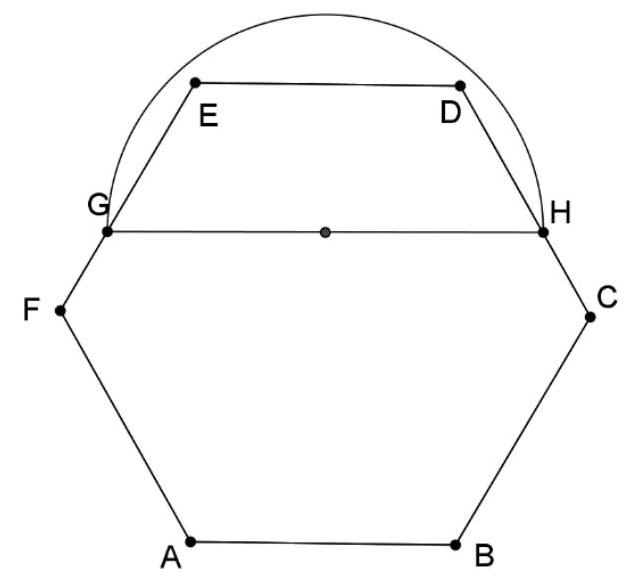
\includegraphics[max width=\textwidth, center]{2024_11_21_ce4f64a1d9a079355499g-1}


\end{document}